\documentclass[11pt,a4paper]{article}

\usepackage[margin=0.5in, top=3cm, bottom=2cm]{geometry}
\usepackage[spanish, activeacute]{babel}
\usepackage[utf8]{inputenc}
\usepackage{amsthm}
\usepackage{amsmath}
\usepackage{amsfonts}
\usepackage{amssymb}
\usepackage{graphicx} %Para incluir el logo de la UBA
\usepackage{caratula} %Para armar el cuadro de integrantes
\usepackage{todonotes}
\usepackage{hyperref}
\usepackage{float}
\usepackage{url}
\usepackage[linesnumbered]{algorithm2e}
\usepackage{minted}

\graphicspath{{imagenes/}}

%Cosas para escribir codigo fuente
%Fuente: http://en.wikibooks.org/wiki/LaTeX/Source_Code_Listings
\usepackage{listings}
\usepackage{color}

\setcounter{secnumdepth}{5}

\begin{document}

\integrante{Vileriño, Silvio}{106/12}{svilerino@gmail.com}
\integrante{Chapresto, Matías}{201/12}{matiaschapresto@gmail.com}
\integrante{Garassino, Agustín}{394/12}{ajgarassino@gmail.com}

\def\Materia{Bases de Datos}
\def\Titulo{Trabajo Pr\'{a}ctico 2}
\def\Fecha{29 de junio de 2015}

%----- CARATULA -----%

\thispagestyle{empty}

\begin{center}
	
\includegraphics[scale = 0.25]{imagenes/logo_uba.jpg}
\end{center}

\begin{center}
	{\textbf{\large UNIVERSIDAD DE BUENOS AIRES}}\\[1.5em]
	{\textbf{\large Departamento de Computaci\'{o}n}}\\[1.5em]
    {\textbf{\large Facultad de Ciencias Exactas y Naturales}}\\
    \vspace{25mm}
    {\LARGE\textbf{\Materia}}\\[1em]    
    \vspace{15mm}
    {\Large \textbf{\Titulo}}\\[1em]
    \vspace{15mm}
    {\textbf{\Large \Fecha}}\\
    \vspace{15mm}
    \vspace{25mm}
    \textbf{\tablaints}
\end{center}

\newpage
\thispagestyle{empty}
\tableofcontents

\parskip=5pt
\setlength{\parindent}{0pt}

\newpage
\setcounter{page}{1}
\pagenumbering{arabic}
\pagestyle{plain}

\section{Introducci'on}
Hoy en día el vertiginoso avance de la tecnología hace que las herramientas que una vez nos fueron útiles deban adaptarse constantemente, para poder seguir cumpliendo su función ante la inevitable concepción de las nuevas problemáticas que estos avances conllevan. Por ejemplo en el ámbito de la informática el crecimiento exponencial del internet vino acompañado del desafío de almacenar grandes volúmenes de información, mucho mayores a los que se venían manejando en décadas pasadas. Si bien ya existían herramientas con este fin, su capacidad no logró cubrir todas las necesidades que se presentaron junto con esta revolución. El objetivo de este documento es plantear, bajo este contexto, los inconvenientes de las bases de datos tradicionales y las ventajas que ofrecen las nuevas para la resolución de este dilema.	

\section{Motivacion para la eleccion del tema}
Nos pareci\'o interesante hacer una investigacion acerca de estos temas, ya que son tecnologias muy nuevas pero al mismo tiempo muy utilizadas en la industria, solucionan ciertas problematicas de las tecnologias utilizadas clasicamente que consideramos importantes para las necesidades actuales de almacenamiento y disponibilidad de informacion en todo tipo de \'ambitos. 

\section{Problemática de las bases de datos relacionales}
Las bases de datos relacionales son aquellas que cumplen con el modelo relacional \footnote{ \href{http://www.seas.upenn.edu/~zives/03f/cis550/codd.pdf}{``A relational model of data for large shared data banks''} Codd, E. F. (1970). }. Este fue uno de los primeros modelos en surgir y es aún el más difundido en la actualidad. Este tipo de bases se desempeñan muy bien a la hora de enfrentar problemas como modificar los datos manteneniendo en todo momento la consistencia de los mismos. Las más utilizadas proveen soluciones inteligentes para respetar las llamadas propiedades ACID \footnote{ \href{http://research.microsoft.com/en-us/um/people/gray/papers/theTransactionConcept.pdf}{``The Transaction Concept: Virtues and Limitations''} Gray, Jim (September 1981).}. Si bien estas propiedades son deseables, no son un requisito excluyente para el funcionamiento de una base de datos bajo determinados contextos. Cuando surgió la necesidad de manejar grandes cantidades de información se comenzaron a utilizar sistemas distribuidos. Es decir, una gran cantidad de computadoras trabajando en conjunto para proveer una interfaz única para el acceso a los datos. Así salió a la luz el hecho de que las herramientas más utilizadas hasta el momento (MySQL, PostgreSQL, etc...) no lograban desarrollar todo su potencial bajo esta nueva arquitectura. Esto se formalizó en el teorema de Brewer también llamado teorema CAP \footnote{ \href{http://webpages.cs.luc.edu/~pld/353/gilbert_lynch_brewer_proof.pdf}{Brewer’s Conjecture and the Feasibility of
Consistent, Available, Partition-Tolerant Web} Gilbert y Lynch (2002)}. El teorema establece la imposibilidad de obtener consistencia, disponibilidad y tolerancia a la partición al mismo tiempo en un sistema distribuido(en particular, una base de datos). La consistencia está relacionada con la misma C que en las propiedades ACID antes mencionadas. La disponibilidad está relacionada con la capacidad del sistema de devolver una respuesta en todo momento, ya sea con la información solicitada o con un error, pero el servicio debe estar disponible. Finalmente la tolerancia a la partición tiene que ver con la misma problemática que nombramos en las bases de datos relacionales: la capacidad de funcionar en múltiples nodos de manera eficiente, no necesariamente en una única computadora.

\section{Bases de datos NoSQL}
Las bases de datos NoSQL surgen como una solución al problema de escalar horizontalmente ante los volúmenes masivos de información que surgieron junto con la popularización de la internet y los nuevos servicios que fueron lanzados. Sacrifican en cierto grado, algunas de las propiedades tradicionales como consistencia, a favor de la capacidad de funcionar en múltiples ordenadores. Esto abre la posibilidad de escalar agregando nuevos nodos al sistema distribuido en el que se encuentra funcionando sin sacrificar disponibilidad. El término NoSQL es utilizado para todas aquellas bases de datos que no siguen el modelo relacional antes mencionado. Estas nuevas bases por lo general proveen una característica denominada consistencia eventual. La consistencia eventual nos asegura que a pesar de que la base de datos sea momentáneamente inconsistente, el estado del sistema se modificará de manera autónoma hasta ser consistente.

El término SQL se refiere a un lenguaje de programación utilizado para interactuar con las bases de datos. Las bases de datos NoSQL no necesariamente proveen la capacidad de interactuar con ellas a través de este lenguaje e incluso pueden tampoco ofrecer alternativas análogas para todas las operaciones permitidas típicamente.

\section{Apache Cassandra}

\subsection{Porque Cassandra?}
\begin{itemize}
  \item \textbf{Arquitectura descentralizada: } Todo nodo dentro del cluster tiene el mismo rol. No existe punto unico de falla(SPOF). Los datos son distribuidos dentro del cluster, con lo cual cada nodo contiene diferentes datos, pero dada esta arquitectura, cualquier nodo puede satisfacer cualquier request.


  \item \textbf{Replicacion en multiples Data-centers: } Cassandra esta disenada como un sistema distribuido, pensado para ser desplegado en un gran numero de nodos a lo largo de multiples data-centers, pensado para mantener redundancia ante la eventual caida de nodos o recuperacion de desastres. Tiene grados configurables de replicacion.

  \item \textbf{Escalable: } El throughput de lecturas y escrituras aumenta linealmente a medida que nuevos nodos se van agregando, sin sufrir \texttt{downtime} ni interrupciones en el servicio. 

  \item \textbf{Tolerante a fallas: } Los datos son automaticamente replicados a multiples nodos para satisfacer esta funcionalidad. Cuando un nodo se cae, es facilmente reemplazable sin sufrir \texttt{downtime}.

  \item \textbf{Multiples niveles de consistencia: } Lecturas y escrituras ofrecen diferentes niveles de consistencia, desde ``las escrituras jamas fallan'' hasta ``bloquear lecturas hasta tener todas las replicas'', con mecanismos de quorum \footnote{ \href{https://en.wikipedia.org/wiki/Quorum_(distributed_computing)}{Tecnicas basadas en quorum para sistemas distribuidos} Wikipedia} como punto intermedio.

  \item \textbf{Interface pseudo-legacy: } Cassandra introduce el lenguaje CQL (Cassandra Query Language) como alternativa parecida a SQL para realizar operaciones \texttt{permitidas}. Tambien estan disponibles drivers de este lenguaje para lenguajes de alto nivel. 
\end{itemize}

\subsection{Modelo}
Apacha Cassandra es una base de datos NoSQL distribuida. El proyecto es de código abierto y está originalmente escrito en Java. Se basa en un modelo de \textit{clave-valor}, utiliza el concepto de contenedores: cada contenedor posee tantos pares de clave y valor como uno quiera. En estos contenedores se guardan ``familias de columnas'' el análogo a las tablas en las bases de datos relacionales. Si las tablas se pueden ver como listas de listas, entonces estas familias se pueden ver como pares (clave, valor) anidados. El análogo a una base de datos es el llamado \textit{KeySpace} o contenedor. Veamos un ejemplo:

\begin{listing}
\begin{minted}[frame=single,
               framesep=3mm,
               linenos=true,
               xleftmargin=21pt,
               tabsize=4]{js}
{
	"user1": {
           "Bio": {
                   "name": "John Smith",
                   "age" : 23
           }
    },
    "user2": {
           "Bio": {
                   "name": "Adam Goldstein",
                   "profession": "Developer"
           },
           "Education": {
                   "bachelors": "Computer Science"
           }
    }
}
\end{minted}
\caption{Pares clave-valor} 
\label{json-example}
\end{listing}

En el ejemplo se puede ver un primer nivel en donde las claves son ID's de usuarios y los valores son a su vez pares de (clave, valor). Para el usuario 1 se tiene la clave Bio que tiene como valor otro conjunto de (clave, valor) anidado albergando nombre y edad. El usuario 2 tiene además de la clave Bio, una clave Education. Como se puede ver la información se encuentra desestructurada y en principio no hay restricciones en cuanto a la forma en que se anidan estas familias de columnas. Bio para el usuario 1 guarda nombre y edad mientras que para el segundo guarda nombre y profesión. El primer nivel de profundidad en estos pares anidados es conocido como filas (user1, user2), el segundo nivel son las familias de columnas (Bio, Education) y finalmente dentro de estas familias se encuentran las columnas. Por cómo es el modelo también se pueden crear estructuras con \textit{super columnas} que es básicamente incrementar el nivel de profundidad de estos pares anidados agregando columnas dentro de las columnas.

Este modelo simple y desestructurado sin embargo tiene sus desventajas. Por ejemplo si uno quisiera ordenar o agrupar por determinado campo, es necesario que este forme parte de la clave para esa fila. Cuando la clave está compuesta por un solo elemento como en el caso de los usuarios (tenía solo los ID's: user1, user2) se llama clave primaria. Cuando la clave está compuesta por múltiples elementos se denomina clave compuesta y se divide en dos partes: la partition key y la clustering key. La partition key es la mínima cantidad de datos que hay que meter en una query para poder obtener las filas deseadas, la clustering key son datos extra que sirven por ejemplo para aprovechar las capacidades de ordenamiento. En el primer ejemplo se tiene una clave simple, por lo tanto es una clave primaria, la mínima cantidad de datos necesaria para obtener una fila es el id del usuario. En el siguiente ejemplo se almacenan empleados en una base de datos y se tiene una clave compuesta por compañía y nombre: la partition key es la compañía y por lo tanto con este alcanza para obtener la fila deseada, la clustering key es el nombre y nos servirá por ejemplo para ordenar. Internamente Cassandra guarda la clustering key como columnas compuestas, como se puede ver en el ejemplo. Como mencionaremos posteriormente la partition key es muy importante para determinar cómo se reparten las filas entre los nodos, es decir cómo se decide qué nodo guarda cada porción de datos.

\begin{table}[h]
\centering
\caption{Contenido}
\label{my-label}
\begin{tabular}{|l|l|l|l|}
\hline
Company & Name & Age & Role \\ \hline
OSC     & Eric & 38  & ceo  \\ \hline
OSC     & John & 37  & dev  \\ \hline
RKG     & Anya & 29  & lead \\ \hline
RKG     & Ben  & 27  & dev  \\ \hline
RKG     & Chad & 35  & ops  \\ \hline
\end{tabular}
\end{table}

\begin{listing}
\begin{minted}[frame=single,
               framesep=3mm,
               linenos=true,
               xleftmargin=21pt,
               tabsize=4]{js}
{
	"OSC": {
           "eric:age": 38,
		   "eric:role": "ceo",
		   "john:age": 37,
		   "john:role": "dev",
    },
    "RKG": {
           "anya:age": 29,
		   "anya:role": "lead",
		   "ben:age": 27,
		   "ben:role": "dev",
		   "chad:age": 35,
		   "chad:role": "ops"
    }
}
\end{minted}
\caption{Pares clave-valor con clave primaria compuesta} 
\label{json-example}
\end{listing}

Hay varias operaciones tradicionales que no están permitidas, por ejemplo un JOIN.

\subsection{¿Cómo almacena Cassandra los datos en los nodos?}
Cassandra reparte los datos uniformemente entre los nodos de un cluster. Generalmente este conjunto de nodos es visualizado como un anillo donde cada nodo tiene dos vecinos. A cada nodo se le asigna la responsabilidad sobre un rango de hashes. Este rango puede ser configurado de diversas maneras, pero la idea general es distribuir los datos de la forma más equitativa posible. Cada update que se le hace a la base de datos para agregar una fila contiene una clave primaria (o partition key en el caso de que sea compuesta), esta clave es hasheada y luego se busca qué nodo dentro del cluster es responsable de ese update en base al resultado. Luego el dato es guardado \textit{n} veces en distintos nodos dentro del cluster, ese \textit{n} es configurado a través del \textit{replication factor} asignado al \textit{keyspace}. Todos los nodos son iguales y las escrituras y lecturas pueden ser realizadas a través de cualquier nodo ya sea este responsable o no del hash de la clave primaria. No hay un nodo maestro. Los nodos aprenden constantemente sobre la estructura general del cluster a través de un protocolo estilo Gossip \footnote{ https://en.wikipedia.org/wiki/Gossip\_protocol } , utilizando una comunicación \textit{peer-to-peer}. El nodo al que se le realiza la consulta o escritura es denominado nodo coordinador. Este nodo encontrará a los nodos responsables para esta acción y una vez que consiga el resultado lo devolverá. \\


\centerline{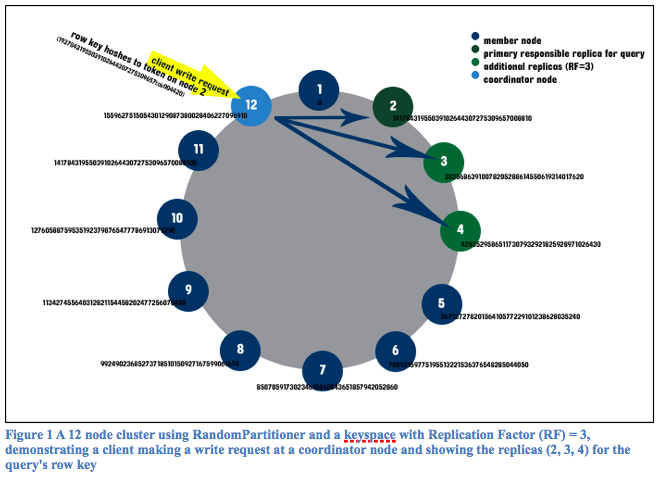
\includegraphics[scale=0.5]{imagenes/cassandra-ring}}

Cuando se realiza un update de una fila primero se guarda la escritura en el commit log, posteriormente se escribe a memoria. Esta tabla es utilizada hasta llegar a su tamaño máximo (que también es configurable) y posteriormente es flusheada a una en disco denominada \textit{SSTable}. Si hay un fallo en alguno de los nodos, los eventos son ejecutados nuevamente desde el commit log para recuperar el estado deseado a pesar de que la tabla en memoria no hubiera sido flusheada a disco. \\

\centerline{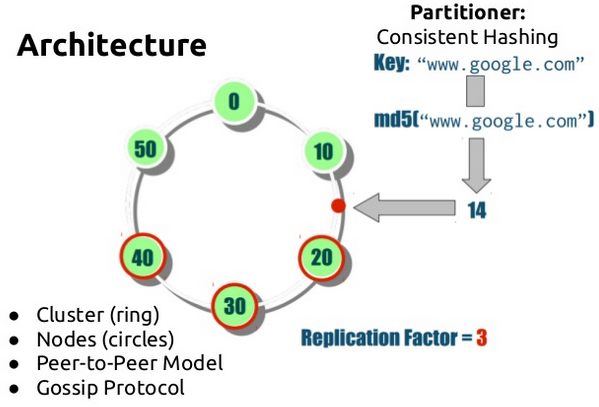
\includegraphics[scale=0.5]{imagenes/cassandra-ring-2}}

\subsection{¿Cómo se hacen las consultas en Cassandra?}

Hay numerosas formas de interactuar con los datos almacenados en la base de datos. La más familiar para los usuarios que provienen de utilizar bases de datos relacionales es sin duda \textit{CQL}. Este lenguaje provee una sintaxis similar a la de \textit{SQL} para realizar un subconjunto de las operaciones de este, recordemos que Cassandra es incapaz de por ejemplo realizar JOINS. Debido a su estructura interna ciertas operaciones pierden sentido y esto implica que la morfología de la base tenga que ser pensada desde otro punto de vista. A la hora de modelar la base de datos se tendrá que tener en cuenta estas limitaciones. Veamos un ejemplo de CQL:

\begin{lstlisting}

CREATE KEYSPACE demo
WITH REPLICATION = { 'class' : 'SimpleStrategy', 'replication_factor' : 1 };

CREATE TABLE users (
  user_name varchar PRIMARY KEY,
  password varchar,
  birth_year bigint
);
 \end{lstlisting}

Primero creamos un \textit{KeySpace} o contenedor en donde almacenar nuestro mapa de (clave, valor). Al hacer esto podemos configurar características como el factor de replicación del que se habló anteriormente y la estrategia que se utilizará para la replicación de las filas \footnote{ \href{http://docs.datastax.com/en/cassandra/2.0/cassandra/architecture/architectureDataDistributeReplication_c.html}{SimpleStrategy}:
Use only for a single data center. SimpleStrategy places the first replica on a node determined by the partitioner. Additional replicas are placed on the next nodes clockwise in the ring without considering topology (rack or data center location).} \footnote{http://blogs.atlassian.com/2013/09/do-you-know-cassandra/} . Si se tienen muchas claves, el orden en el que se declaran es importante por que determinará cuáles corresponderán a la partition key y cuáles a la clustering. Esto también se puede indicar de manera explícita para no depender del orden.

Posteriormente se crea una ``tabla'' que en realidad Cassandra internamente guarda dentro de su KeySpace de la siguiente forma, teniendo en cuenta los siguientes datos:

\begin{table}[h]
\centering
\caption{Tabla con datos al estilo ``relacional''}
\label{my-label}
\begin{tabular}{|l|l|l|l|}
\hline
user\_name & password & birth\_year \\ \hline
pepe1      & asdasd   & 1990        \\ \hline
robert18   & qweqwe   & 1987        \\ \hline
\end{tabular}
\end{table}

\begin{listing}
\begin{minted}[frame=single,
               framesep=3mm,
               linenos=true,
               xleftmargin=21pt,
               tabsize=4]{js}
{
	"pepe1": {
           "password": "asdasd",
		   "birth_year": "1990"
    },
    "robert18": {
           "password": "qweqwe",
		   "birth_year": "1987"
    }
}
\end{minted}
\caption{Mapeo de tabla en modelo relacional a Cassandra según CQL} 
\label{json-example}
\end{listing}

\begin{lstlisting}
INSERT INTO users (user_name, password, birth_year)
VALUES ('john46', 'zxczxc', '1991');

SELECT * FROM users WHERE user_name= 'john46';
\end{lstlisting}

Insertar valores y obtenerlos es similar a SQL también. Recordemos que para hacer cualquiera de estas operaciones es necesario como mínimo pasar el conjunto de elementos dentro de la partition key en la consulta. Es decir, como mínimo se necesitan los elementos para que el nodo coordinador pueda hashear la entrada y obtener la dirección del nodo que se debe encargar de hacer la réplica principal y en base a este quiénes se encargarán de hacer las redundantes.

También se pueden encontrar abstracciones y drivers para distintos lenguajes de más alto nivel, por ejemplo utilizando querysets a través de python \footnote{http://datastax.github.io/python-driver/cqlengine/queryset.html}.

\subsection{Casos de uso}

\subsubsection{Puntos fuertes}
Uno de los puntos fuertes de esta base de datos es la escalabilidad lineal en función de los nodos, uno puede agregar tantos como necesite hasta obtener la capacidad deseada sin inconvenientes ni interrupción del servicio. La naturaleza distribuida de esta base de datos no le da más importancia a ninguno de los nodos por los cuales está constituida, no posee ningún nodo maestro y además utiliza protocolos peer-to-peer para la comunicación entre ellos. Esto sumado a que posee cierta redundancia de la información entre los distintos nodos la hace una base bastante robusta y resistente frente a la posible caida de alguno de los nodos.

Todas estas características la hacen una herramienta ideal para el problema que se mencionó al principio del documento: la escalabilidad frente a un flujo masivo de datos, en un contexto donde la consistencia no es un requisito en todo momento. Un contexto donde la consistencia eventual, propagando la información a través de los nodos a lo largo del tiempo es suficiente. A diferencia de las bases de datos relacionales los \textit{write} son muy baratos, y si los datos se distribuyen uniformemente y de manera equitativa entre todos los nodos del anillo, entonces los \textit{read} también lo serán. Veamos a continuación algunos ejemplos de la vida real.

\subsubsection{eBay}
El conocido servico de compra-venta utiliza Cassandra para servir varios de sus datos: social signals en sus productos, grafo de gustos para recomendar productos a sus usuarios, notificaciones móviles, etc. Por otro lado no la utilizan para otros casos de uso como Big Data. Algunas características del deploy de Cassandra de eBay son: más de 200 TB de información, más de 400 millones de writes por día y más de 100 millones de reads por día. \footnote{http://www.slideshare.net/jaykumarpatel/cassandra-at-ebay-13920376}

\subsubsection{Netflix}
El relativamente nuevo servicio de streaming de contenido utiliza Cassandra para almacenar las interacciones entre los subscriptores y sus contenidos descargados. Necesita poder manejar bases de datos distribuidas por todo el planeta(mas de 40 paises). En las fuentes se presenta una diapositiva explanatoria en detalle acerca de la migracion del datacenter relacional a cassandra.
\footnote{http://www.slideshare.net/adrianco/migrating-netflix-from-oracle-to-global-cassandra}

\subsubsection{Otros}

\begin{itemize}
  \item \href{http://live-pc-development.pantheon.io/blog/analytics-at-github-with-apache-cassandra/}{GitHub}
  \item \href{http://www.planetcassandra.org/blog/interview/facebooks-instagram-making-the-switch-to-cassandra-from-redis-a-75-insta-savings/}{Instagram}
  \item Y muchos más en el sitio oficial de \href{http://cassandra.apache.org/}{Apache Cassandra}.
\end{itemize}

\end{document}
